Profilowanie kodu jest kluczowym etapem w procesie optymalizacji. W tej sekcji przedstawimy i omówimy narzędzia dostępne w środowisku Unity do analizy wydajności kodu, a także skonfigurujemy profiler w celu efektywnego monitorowania wydajności. \\ \\
Unity udostępnia zaawansowane narzędzia do profilowania kodu, pozwalające na analizę wydajności w różnych aspektach. Poniżej przedstawiamy kluczowe narzędzia wbudowane w Unity:

\begin{itemize}
    \item \textbf{Profiler Unity} - Profiler to narzędzie, umożliwiające śledzenie i analizę wydajności podczas działania gry lub z okna edytora po przełączeniu trybu na \textit{Edit Mode}. Pozwala ono na monitorowanie zużycia zasobów, czasu renderowania, czasu CPU, alokacji pamięci i innych parametrów, których widoczność możemy przełączać klikając w \textit{Profiler Modules} w oknie Profilera.
    \begin{figure}[h]
        \centering
        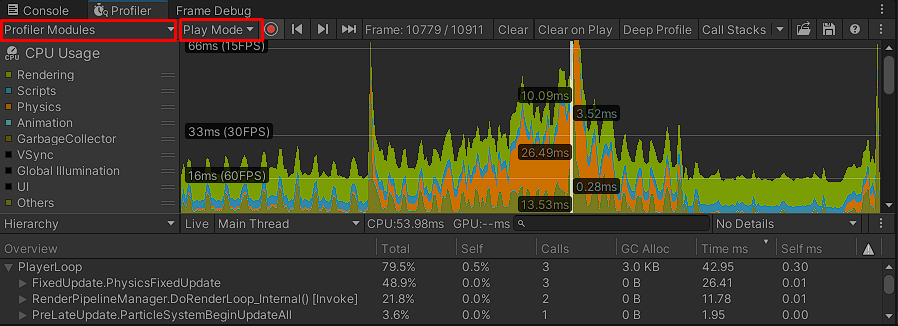
\includegraphics[width=1\linewidth]{Images/unityProfiler.png}
        \caption{Okno Profilera dostępne w menu kontekstowym Window/Analysis/Profiler}
    \end{figure}
    \item \textbf{Unity Frame Debugger} - Frame Debugger pozwala na dokładną analizę, jak Unity renderuje każdą klatkę. Wystarczy kliknąć przycisk \textit{Enable} w oknie Frame Debug i wybrać interesującą nas klatkę. To narzędzie jest szczególnie przydatne do identyfikacji problemów związanych z grafiką i renderowaniem.
    \begin{figure}[h]
        \centering
        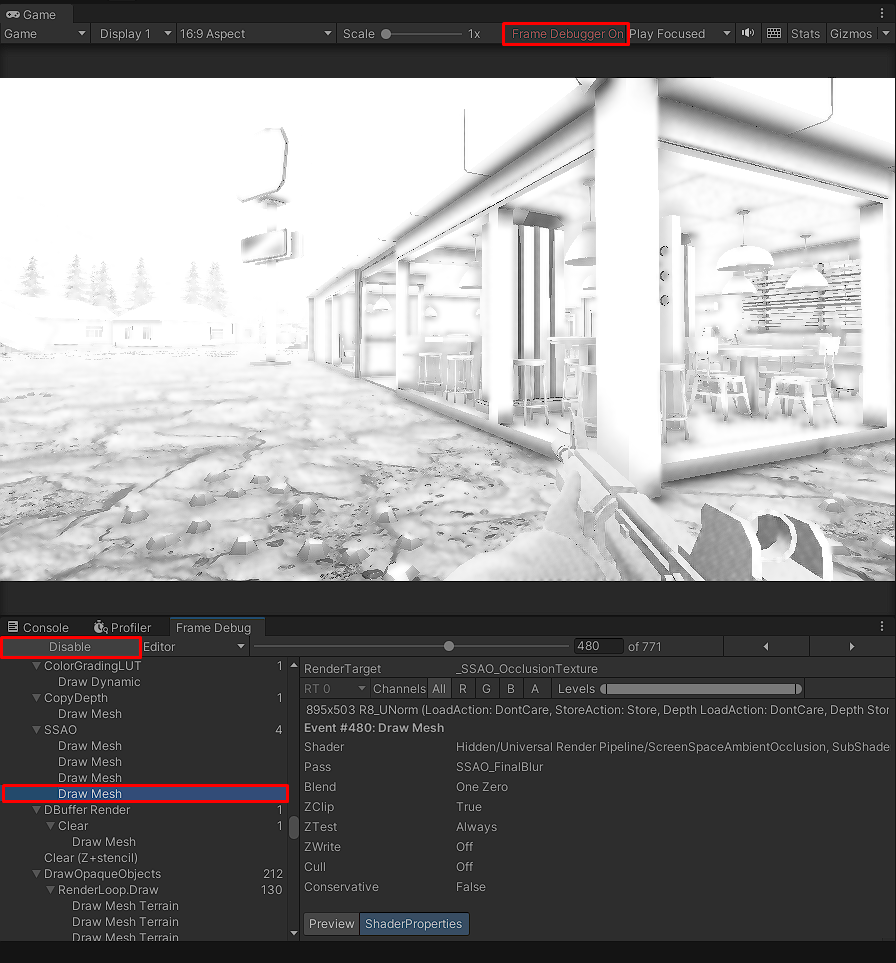
\includegraphics[width=1\linewidth]{Images/frameDebugger.png}
        \caption{Okno Frame Debug, które znajdziemy w menu kontekstowym Window/Analysis/Frame Debugger}
    \end{figure}
    \FloatBarrier
\end{itemize}